\documentclass[12pt,titlepage]{amsart}
\title{An $\alpha$-$\beta$ Monte-Carlo Engine for the Game of Hex}
\author{Eric Vaitl\\November 20, 2017\\CSCI 6550}
\usepackage[margin=1in]{geometry} % margins
\usepackage{placeins} % floatbarrier
\usepackage{setspace} % double spacing
\usepackage{listings} % code listings
\usepackage{hyperref} % \url
\usepackage{havannah} % hex boards
\doublespacing
\begin{document}

\begin{abstract}

    This paper presents an $\alpha-\beta$ game engine with a simple Monte-Carlo
    heuristic for the game of Hex. A sample implementation was written and is
    attached in the appendix. Other approaches and heuristics are discussed and
    compared.

\end{abstract}

\maketitle

\section{Introduction}

First, we'll introduce the rules of hex, some mathematical background, and the
history of the game.

Next, is a walk-though of the interesting portions of the code: The $\alpha-\beta$
routine, the child search, and the evaluation heuristic used.

\section{The Game}

The game is played on a rhombus board made of hexagons:

\begin{HexBoard}[board size=5]
\end{HexBoard}

The standard size for game play is 11x11.  This is a turn based game. Each turn
the player gets to occupy one new currently unoccupied location. The object for
each player is to connect the two sides of the player's color by occupying a
connecting set of locations to form a chain \cite{Maarup05}.

Because the first player has a distinct advantage, some versions of the game
have a \emph{swap rule}. If the swap rule is in effect, the second player can
swap places with the first player right after the first player makes his first
move. This forces the first player to make an inferior first move or play at a
disadvantage.

In the task environment classification scheme used in \cite{RN:AIAMA:2003}, Hex
is a fully observable, multi-agent, deterministic, sequential, static, discrete
game.

\section{History}

Hex is a simple game and has been ``discovered'' at least twice. In 1942-1943
Piet Hein wrote a number of columns about Hex, which he called Polygon, in the
Danish newspaper \emph{Politiken}. Hein had a printer print up small books of
empty Hex sheets for sale. They were advertised for among other things, as a
diversion while spending a night in the public bomb shelters. The newspaper
columns petered out in mid 1943, either because of loss of interest or because
of more pressing issues (Hein's wife was Jewish).

In 1949 John Nash independently invented the game while he was a graduate
student at Princeton \cite{Nash:1952:Games}. Apparently the game became quite
popular among the other students after one of the graduate students created a
Hex board that was available in the Fine Hall common room.

At Princeton and later at Bell Labs, John Nash worked with Claude Shannon.
Shannon created an electrical analog machine that played Hex pretty well. The
board was set up as a resistance network with resistances changed based on the
moves made. The next move was made to the position with the highest voltage
drop.

Shannon's Hex machine work was well before the 1956 Dartmouth conference, which
is often regarded as the birth of AI. However, the cold war was in effect and
people working with the new electronic computers were overly optimistic about
what could be done with the simple schemes available. I thought the closing
paragraph  of \cite{Nash:1952:Games} was quite enlightening:

\begin{quote}
If a military engagement be regarded as a game, such an approach might be useful
in suggesting an overall strategy. Of course, it is not probable that any analog
method quite as simple as those described above would be very useful for most
military applications.
\end{quote}

In 1953 Parker Brothers released Hex as a board game. Unfortunately it is
currently out of print. Hugo Piet Hein, son of Piet Hein, has a little company
that is selling Hex boards today \footnote{\url{http://www.hexboard.com/}}.

Hex has appeared several times in the Computer Olympiads between 2000 and 2011.
The last computer champion was MoHex in 2011 \cite{Henderson:2010}.

\section{Math}

Quite a bit of theory from different domains applies to Hex. Game theory,
algebraic topology, AI, and computational complexity theory are some of the
areas that have been used to analyze this simple game.

Draw a square and color two opposite sides white and the two remaining sides
black. Something that seems obvious is that if you connect two sides of the same
color with an interior line, it is not possible to also connect the remaining
two sides with an interior line unless the two lines cross.  However, the
definitive proof requires the Four Color Theorem from topology.

A less obvious result is that if you fill the central square with the two colors
at least one pair of sides must be connected by a continuous line of the same
color. The easiest known proof of this seems to involve the Brouwer Fixed-Point
Theorem of algebraic topology \cite{Gale:1980} and didn't happen until 1979. An
earlier, longer proof the Jordan Curve Theorem seems to have been discovered in
1969.

So, topology gives us two results for a completed Hex game:
\begin{itemize}
\item In a completed Hex board one pair of sides must be connected.

\item In a completed Hex board, if one pair of sides are connected, the other
pair is not.
\end{itemize}

With both results, we can say that there are no draws. One side will win and the
other side will lose.

John Nash assumed without a complete proof that there were no draws as a given
in 1949 and used a strategy stealing argument from Game Theory (which is a field
he largely invented) to prove that with perfect play the first player in a Hex
game would always win.  His proof was by contradiction: An extra piece on the
board never makes your position worse. Assume with perfect play the second
player could win. The first player could place one piece then play as the second
player to win. This contradicts the second player winning, so with perfect play
the first player must win.

In terms of time, the best known algorithms for solving Hex are intractable (no
polynomial time solution). However, in terms of space, if we had an oracle to
tell us if a position was winnable by white, we could save the perfect play game
tree in polynomial space.  In computational complexity theory, PSPACE is the set
of decision problems that can be solved in a polynomial amount of space. It
turns out that Hex is not only a PSPACE problem, but was shown in 1981 to be
PSPACE complete \cite{Reisch1981}. This means that any other PSPACE problem can
be reduced in polynomial time to an equivalent Hex game of some size.


\section{The Program}
\FloatBarrier

The code is written in C++11, but I'm compiling with C++14 with GNU extensions.
It has been tested with both g++ 7.2.0 and clang++ 5.0.0 on my Linux box
(manjaro).

On invocation, you can optionally specify the board size, search depth, and
branching factor.

\subsection{$\alpha-\beta$}

The $\alpha-\beta$ algorithm is implemented in listing \ref{lst:ab}. It is a bit
more complicated than the reference $\alpha-\beta$ algorithm in
\cite{RN:AIAMA:2003} because there are a few more details that have to be taken
care of in real code.

We don't just need the value of the search tree, but we need the actual move to
make. We could do that with a global that is set before a return and count on
the top level call returning last, but I am allergic to globals and decided to
return a C++ \texttt{pair$<$value,move$>$} instead. The pair is aliased with the
C++11 \texttt{using} directive to both \texttt{opens\_elem} and
\texttt{alpha\_beta\_value}. A good argument could be made that we should use
the same typename for both cases, but I wasn't sure of that when I was writing
the code.

It isn't normally possible to evaluate the full tree, so we pass a
\texttt{depth} parameter that is decremented on each recursive call. When the
depth reaches 0, we just return the \texttt{leaf\_eval} of the node and set the
move to an illegal value (-1).

The same function is used for both minimum and maximum nodes. The boolean
\texttt{maximize} parameter is used to differentiate between the two.
\texttt{maximize} is passed to \texttt{find\_children} to sort and select
children nodes and is used locally to determine if we are comparing with
$\alpha$ or $\beta$.

\singlespacing
\begin{lstlisting}[language=C++,float,label={lst:ab},basicstyle=\small,
                   caption=$\alpha-\beta$]
alpha_beta_value alpha_beta(int depth,
                            bool maximize,
                            double alpha,
                            double beta){

    node_state next_turn = maximize ? node_state::HUMAN : node_state::COMPUTER;
    board &b = *pb;

    vector<opens_elem> opens = find_children(depth, maximize);

    //    If there are no children or we are at our search depth, just return
    //    current eval.
    if (depth <= 0 || opens.size() == 0) {
        return alpha_beta_value(leaf_eval(b, next_turn), -1);
    }
    // We now have up to branch-size children to check.
    double v = maximize ? -numeric_limits<double>::max() :
               numeric_limits<double>::max();
    int move = 0;
    for (auto m: opens) {
        int idx = m.second;
        b(idx) = maximize ? node_state::COMPUTER : node_state::HUMAN;
        auto ab = alpha_beta(depth - 1, !maximize, alpha, beta);
        if (maximize) {
            if (ab.first > v) {
                move = idx;
                v = ab.first;
            }
            alpha = max(alpha, v);
        }else{
            if (ab.first < v) {
                move = idx;
                v = ab.first;
            }
            beta = min(v, beta);
        }
        b(idx) = node_state::OPEN;
        if (beta <= alpha) {
            break;
        }
    }
    return alpha_beta_value(v, move);
}
\end{lstlisting}
\doublespacing
\subsection{find\_children}

The \texttt{find\_children} implementation is in listing \ref{lst:fc}.

Like the game Go, Hex can have a very large branching factor. On an NxN board,
the branch factor starts at $N^2$ and decreases by 1 for each move.

The branching factor for searching is set by the global \texttt{branch\_factor},
which I justify because it is set just once at program startup.
\texttt{find\_children} returns the best (or worst) \texttt{branch\_factor}
candidates based on the boolean \texttt{maximize}.

I left open the possibility of two different evaluation functions depending on
whether we are evaluating a leaf (\texttt{leaf\_eval}) or choosing interior
children for branching (\texttt{branch\_eval}). The current program actually
uses the same evaluation function for both.

After evaluating all children of the current node, the top
\texttt{branch\_factor} children of an interior node are selected and returned.
If we are in a leaf node (because \texttt{depth}$\leq 1$), then just one node is
selected and returned.

Sorting is inlined using C++11 lambda functions, which are passed to the
standard template \texttt{sort} routine. The use of \texttt{vector} instead of
traditional C arrays makes memory management much easier. C++11 r-value
references makes passing vectors much more efficient than they were in pre-C++11
days.

\singlespacing
\begin{lstlisting}[language=C++,float,label={lst:fc},
                   basicstyle=\small,caption=find\_children]
vector<opens_elem> find_children(int depth, bool maximize){
    board &b = *pb;
    int size = b.size();

    vector<opens_elem> opens;
    auto sortfn = maximize ?
                  [](opens_elem p1, opens_elem p2) {
                      return p1.first > p2.first;
                  } :
                  [](opens_elem p1, opens_elem p2) {
                      return p1.first < p2.first;
                  };
    auto eval = depth <= 1 ? leaf_eval : branch_eval;
    for (int idx = 0; idx < size * size; ++idx) {
        if (b(idx) == node_state::OPEN) {
            b(idx) = maximize ? node_state::COMPUTER : node_state::HUMAN;
            double e = eval(b,
                            (maximize ? node_state::HUMAN :
                             node_state::COMPUTER));
            b(idx) = node_state::OPEN;
            opens.push_back(opens_elem(e, idx));
        }
    }
    sort(opens.begin(), opens.end(), sortfn);
    if (depth <= 1) {
        opens.resize(min(1, int(opens.size())));
    } else{
        opens.resize(min(branch_factor, int(opens.size())));
    }
    return opens;
}
\end{lstlisting}
\doublespacing
\subsection{eval}

The evaluation function for this program is the function \texttt{rwins} in
Listing \ref{lst:eval}. It is almost stupidly simple. It fills out the board as
if two idiots were playing \texttt{MC\_TIMES} and saves the percent of time the
first player wins. The result is scaled from 1 to -1. If the computer wins every
time, the result is 1, if the human wins every time, the result is -1.

The \texttt{check\_winner} class is a little more complicated. It does a depth
first search of the board from each of the first columns and sees if any
location in the last column is reachable from a location in the first column.  I
had considered using a union-find, but the depth first searching seems as fast
in practice.

\singlespacing
\begin{lstlisting}[language=C++,float,
                  label={lst:eval},basicstyle=\small,
                  caption=Evaluation Function]
static double rwins(const board &b,
                    node_state next_turn = node_state::COMPUTER){
    int wins{ 0 };

    for (int i = 0; i < MC_TRIALS; ++i) {
        board lb(b);
        fill_board(lb, next_turn);
        if (check_winner(lb).winner() == winner_state::COMPUTER) {
            ++wins;
        }
    }
    return (wins - MC_TRIALS / 2.0) / MC_TRIALS;
}
\end{lstlisting}
\doublespacing

\FloatBarrier
\section{Sample Play}

Here is a sample play with a board size of 4, search depth of 4, and branching
factor of 5.

For such a simple program, it is a surprisingly good player. A single mistake by
the human player is usually enough to cause a loss.:

\singlespacing
\begin{verbatim}
    $ ./hex -s 4 -d 4 -f 5
                 C
         1   2   3   4
       1 . - . - . - .
          \ / \ / \ / \
         2 . - . - . - .
            \ / \ / \ / \
      H    3 . - . - . - .  H
              \ / \ / \ / \
             4 . - . - . - .
               1   2   3   4
                       C
    Input space separated row and column: 2 2
                 C
         1   2   3   4
       1 . - . - . - .
          \ / \ / \ / \
         2 . - H - C - .
            \ / \ / \ / \
      H    3 . - . - . - .  H
              \ / \ / \ / \
             4 . - . - . - .
               1   2   3   4
                       C
    Input space separated row and column: 3 3
                 C
         1   2   3   4
       1 . - . - . - .
          \ / \ / \ / \
         2 . - H - C - .
            \ / \ / \ / \
      H    3 . - C - H - .  H
              \ / \ / \ / \
             4 . - . - . - .
               1   2   3   4
                       C
    Input space separated row and column: 1 4
                 C
         1   2   3   4
       1 . - . - C - H
          \ / \ / \ / \
         2 . - H - C - .
            \ / \ / \ / \
      H    3 . - C - H - .  H
              \ / \ / \ / \
             4 . - . - . - .
               1   2   3   4
                       C
    Input space separated row and column: 4 2
                 C
         1   2   3   4
       1 . - . - C - H
          \ / \ / \ / \
         2 . - H - C - .
            \ / \ / \ / \
      H    3 . - C - H - .  H
              \ / \ / \ / \
             4 C - H - . - .
               1   2   3   4
                       C
    winner: computer
\end{verbatim}
\doublespacing

\section{Other Heuristics}

The traditional heuristic is that resistance netowork used by Shannon. It may
however  be a bit harder to implement in software than in hardware. While
writing the code for this project, I looked at the source code for Wolve, which
was the 2008 Computer Olympiad winner for Hex. When more advanced searches and
pattern matches fail, Wolve falls back to a resistance measure. Wolve uses a
non-standard linear algebra library which makes a best guess when trying to
solve for an under-specified set of linear equations.  Unfortunately, Wolve
doesn't seem to go through the work required to get the independent equations,
so the results it gets from the resistance heuristic are suspect.

The graphical equivalent of

\begin{HexBoard}[board size=5]
\end{HexBoard}

is

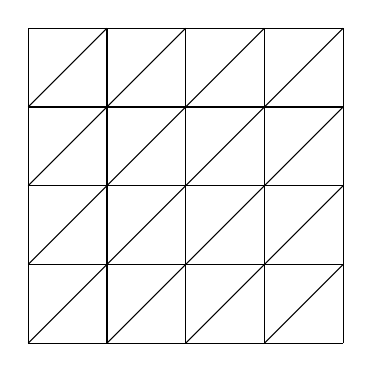
\begin{tikzpicture}
    \draw[step=1cm] (-2,-2) grid (2,2);
    \draw (-2,-2) -- (2,2);
    \draw (-2, -1) -- (1, 2);
    \draw (-2, 0) -- (0, 2);
    \draw (-2, 1) -- (-1, 2);
    \draw (-1, -2) -- (2, 1);
    \draw (0, -2) -- (2, 0);
    \draw (1, -2) -- (2, -1);
\end{tikzpicture}

We assume each edge has a resistance. In order to properly to properly calculate
the resistances in a large mesh network like this, we need to use Kirchoff's
voltage and current laws to generate enough linearly independent equations to
span the space. With $|E|$ edges in a fully connected graph, we need $|E|+1$
linearly independent equations \cite{Moody2013}. Kirchoff's current law states
that the sum of the currents for a vertex is 0. With a graph $G=(V,E)$, that
gets us $|V|$ equations.

Kirchoff's voltage law says the sum of the voltages around a loop is 0. To get
the remaining equations, we start by creating a minimum spanning tree. The edges
not in that tree will each be part of an independent cycle. For each edge not in
the minimum spanning tree we walk up from the parents of the vertices in the
spanning tree until we find a common parent. The set of vertices now form a
loop. Because in a fully connected graph $G=(V,E)$ we have $|V|-1$ edges in the
spanning tree, this spanning tree procedure will give us $|E|-(|V|-1)$ new
equations. Added to the $|V|$ equations we generated from the current law, we
have the required $|E|+1$ linearly independent equations to solve the resistance
network.

With an NxN Hex board plus the required source and sink, there are a total of
$3\times(N-1)^2+2N-1 + 2N$ edges. For the standard 11x11 board, that would
require solving a system of 343 linearly independent equations. This is not a
trivial amount of work for evaluating a single position.

\cite{ANSHELEVICH2002101} describes a heuristic that finds cell-to-cell loose
linkages that work better than straight-forward resistance heuristics. Here is
an example:

\begin{HexBoard}[board size=5]
\HStoneGroup[color=black]{b2,c3}
\end{HexBoard}

The stones at b2 and c3 are linked in that if white tries to block the
connection by placing at either b3 or c2, black can play the other location to
complete the link. The pattern matching for these linkages has become called
H-search. H-search is the primary heuristic used by Six, Wolve, and MoHex, which
were the winners of the Computer Olympiad Hex competitions from 2006 through
2010.

Monte-Carlo has been used in conjunction with $\alpha-\beta$
\cite{arneson_hayward_henderson_2010}, but it is normally used for either
selection or for leaf evaluation, not for both. Most commonly, Monte-Carlo is
used for branch selection, where it is called Monte Carlo Tree Search (MCTS).

The Hex program presented here has hooks for multiple evaluations functions, but
uses the same Monte-Carlo for both leaf and branching evaluation. A more
expensive leaf evaluation, like H-search or resistance should bring the current
program closer to the level of play of the previous Computer Olympiad players.
The big difference will be the opening book and dead region elimination done by
Wolve and in particular MoHex.

\section{Other Approaches}

The current gold standard for a Hex type game is probably AlphaGo Zero
\cite{Silver2017}. Instead of a Monte-Carlo roll-out, AlphaGo Zero used a single
neural network for both position evaluation and branch selection. The neural
network is trained with an MCTS, but the MCTS branch probabilities are guided by
the position valuation of the initial neural network. After 40 days of
continuous self-play AlphaGo Zero was able to beat AlphaGo-Lee 100 games to 0.
AlphaGo-Lee is the program that defeated the human world champion in 2016. An
intermediate program called AlphaGo-Master beat a field of the strongest
professional Go players 60 games to 0. Against AlphaGo-Zero, a 100 game match
was 89/11 in favor of AlphaGo-Zero.

The Machine Learning class was full this semester, but if I can get into it next
year, I may try my hand at using a neural network for the heuristic function.

\section{Future Work}

Obviously, the game needs a GUI. The code is C++ and I work on Linux, so I think
a Qt GUI \cite {Blanchette:2006} would work well. Qt is a C++ GUI framework that
is portable to Linux, Mac, Windows and Android.

It is a bit embarrassing today that the engine is single threaded. I think a
useful architecture for this project may be a single master thread that handles
user input and game play and a number of worker threads (based on the number of
cores available) that would do position evaluation. Other architectures, of
course, are also possible.

While basic thread support has been added to C++11 with \texttt{$<$thread$>$},
The asio \footnote{\url{https://think-async.com/Asio}} library provides a higher
level framework and is quite likely to be part of the C++17 standard. If
somebody wants to get serious about this, the asio framework would allow one to
distribute worker threads across multiple cores or multiple machines for large
scale scaling.

Iterative deepening with a timer would be a large improvement over statically
picking the search depth and branching factor.

Other heuristic functions, such as network resistance, edge current, or neural
network evaluation should be tried.

To test one heuristic against another, a way should be added for two programs to
play each other.

\section{Conclusion}

A basic game engine for Hex can be written in just a couple of hundred lines of
code and can play a decent game. If AI is defined as stuff we don't really know
how to get a computer to do yet, then at this level Hex is more of an
engineering or coding problem than an AI problem.



\bibliographystyle{apalike}
\bibliography{csphd}
\appendix
\section{Code Listing}

The source code is online at \url{https://github.com/evaitl/hex}. It is included
below for completeness.

\singlespacing
\lstinputlisting[language=C++,basicstyle=\small]{hex.cpp}
\end{document}
